\documentclass[a4paper]{IEEEtran}
\usepackage{amsmath}
\usepackage{amssymb}
\usepackage{amsthm}
\usepackage{enumerate}
\usepackage[shortlabels]{enumitem}
\usepackage{algorithm}
\usepackage{algpseudocode}
\usepackage{graphicx}
\usepackage{subcaption}

\newtheorem{definition}{Definition}
\newtheorem{lemma}{Lemma}
\newtheorem{theorem}{Theorem}

%opening
\title{Using PCA on EEG Data to Distinguish Sleep~Stages}
\author{\IEEEauthorblockN{Ida Hönigmann}
	\IEEEauthorblockA{\\Technical University Vienna, Austria\\
		Email: e12002348@student.tuwien.ac.at}}

\begin{document}

\maketitle

\begin{abstract}
[TODO]
\end{abstract}

\section{Introduction}
\label{sec:introduction}

[TODO general introduction]

\subsection{EEG Data and Sleep Stages}

Ganong~\cite{Ganong1997} describes typical patterns observed in electroencephalogram (EEG) data of a sleeping person. He describes the EEG patterns associated with rapid eye movement~(REM) sleep and non-REM~(NREM) sleep.

NREM sleep is further partitioned into four (although some only use three) stages, termed Stage~1 (S1) to Stage~4 (S4). Example EEG data of these different sleep stages can be seen in Figure~\ref{pic:TODO} [TODO image]. The EEG data of these stages is characterized as follows:

\begin{enumerate}[label={S\arabic*:}]
\item low-amplitude, high-frequency
\item appearance of sleep spindles (bursts of higher amplitude, lower frequency waves)
\item increased amplitude, lower frequency
\item maximal amplitude, minimal frequency
\end{enumerate}

In REM sleep the EEG data is that of high frequency and low amplitude patterns, resembling the data observed in alert humans.

\section{Study of Literature}
\label{sec:study_of_literature}

A substantial body of scientific research has been devoted to exploring Principal Component Analysis (PCA).
The foundation of this method was laid by Pearson~\cite{Pearson1901} and Hotelling~\cite{Hotelling1933}.

An introduction to PCA, as well as a good overview on how to derive the formula used to compute the Principal Components (PC) is given by Shlens~\cite{Shlens2014}.
Recent applications and variants of PCA are explored by Jolliffe et. al.~\cite{Jolliffe2016}.

Shlens discusses the limitations of PCA, as well as examples in which PCA fails~\cite{Shlens2014}, such as the requirement of linearly dependent data.
Tenenbaum proposes a non-linear method to combat this problem\cite{Tenenbaum2000}.

Generally speaking the variables must not have third or higher order dependencies\footnote{e.g. $\mathbb{E}[x_ix_jx_k] \neq 0$ for some $i, j, k$ assuming mean-free variables} between them. In some cases it is possible to reduce a problem with higher order dependencies to a second order one by applying a non-linear transformation beforehand. This method is called kernel PCA\cite{Shlens2014}.

Another method for combating this problem is Independent Component Analysis (ICA) which is discussed by Naik~et.~al.\cite{Naik2011}.
\\
\\
The given problem of distinguishing sleep stages given some EEG data has been investigated by use of PCA, as well as neural networks. Some of these works are summarized below.

A review of different methods in the preprocessing, feature extraction and classification is given by Boostani et. al.\cite{Boostani2017}. They find that using a random forest classifier and entropy of wavelet coefficients as feature gives the best results.

Tăuţan et. al.\cite{Tautan2021} compare different methods of dimensionality reduction on EEG data, such as PCA, factor analysis and autoencoders. They conclude that PCA and factor analysis improves the accuracy of the model.

Putilov\cite{Putilov2015} used PCA to find boundaries between Stage~1, Stage~2 and Stage~3. Changes in the first two PC were related to changes between the Stage~1 and Stage~2, while changes in the fourth PC exhibited a change in sign at the boundary of Stage~2 and Stage~3. This suggests that changes between Stage~1 and Stage~2 are easier to detect that ones between Stage~2 and Stage~3.

Metzner et. al.\cite{Metzner2023} try to rediscover the different human-defined sleep stages. They find that using PCA on the results makes clusters apparent. These clusters could then be used as a basis for a redefinition of sleep stages.

The PhysioNet/Computing in Cardiology Challange 2018 was a competition using a similar data\cite{Ghassemi2018}. The goal was to identify arousal during sleep from EEG, EOG, EMG, ECG and SaO2 data given. The winning paper of this competition describes the use of a dense recurrent convolutional neural network (DRCNN) consisting of multiple dense convolutional layers, a bidirectional long-short term memory layer and a softmax output layer\cite{Howe2018}.
\\
\\
As shown in this section, the utilization of PCA to analyze EEG data has been used with success.

\section{Mathematical Basics}
\label{sec:mathematical_basics}

We define mathematical notation, which will be used in Section~\ref{sec:principal_component_analysis} to define the PCA.

\subsection{Covariance}
Assume we have two sets of $n$ observations of variables with mean 0. Let us call the first list of observations $\mathbf{a} = (a_1, ..., a_n)$ and the second $\mathbf{b} = (b_1, ..., b_n)$.

\begin{definition}[covariance]
Let us define the \textit{covariance} of $\mathbf{a} \in \mathbb{R}^n$ and $\mathbf{b} \in \mathbb{R}^n$ as
\begin{align*}
	\sigma_{\mathbf{ab}} := \frac{1}{n} \sum_{i=1}^{n}a_ib_i = \frac{1}{n}\mathbf{a}\cdot\mathbf{b}^T.
\end{align*}
\end{definition}

From the definition it is obvious that the covariance is symmetric, $\sigma_{\mathbf{ab}} = \sigma_{\mathbf{ba}}$. In the special case $\mathbf{a} = \mathbf{b}$ the covariance $\sigma_{\mathbf{aa}}$ is called \textit{variance} $\sigma_{\mathbf{a}}^2$.

\begin{definition}[covariance matrix]
Generalizing to $m$ variables $\mathbf{X} = [\mathbf{x_1}, ..., \mathbf{x_m}]$, each having been observed $n$ times, gives us the \textit{covariance matrix}.

\begin{align*}
	\mathbf{C_X} := \left(\begin{matrix}
		\sigma_{\mathbf{x_1x_1}}	& \cdots & \sigma_{\mathbf{x_1x_m}}	\\
		\vdots						& \ddots & \vdots					\\
		\sigma_{\mathbf{x_mx_1}}	& \cdots & \sigma_{\mathbf{x_mx_m}}	\\
	\end{matrix}\right) = \frac{1}{n} \mathbf{X}\mathbf{X}^T
\end{align*}
\end{definition}

The covariance matrix is a symmetric $m\times m$ matrix.

\subsection{Diagonalizable Matrix}

\begin{definition}[Diagonalizable Matrix]
	A square matrix $\mathbf{A}$ is called \textit{diagonalizable}, if there exists a invertable matrix $\mathbf{P}$ and a diagonal matrix $\mathbf{D}$ such that $\mathbf{A} = \mathbf{P}\mathbf{D}\mathbf{P}^{-1}$.
\end{definition}

\begin{definition}[Symmetric matrix]
	A square matrix $\mathbf{A}$ is called \textit{symmetric}, if $\mathbf{A}^T = \mathbf{A}$.
\end{definition}

\begin{theorem}
	\label{th:symmetric_matrix_diagonalizable}
	Every symmetric matrix is diagonalizable.
\end{theorem}

The proof of this theorem requires some preparation, which we will do now.

\begin{definition}[Eigenvalues and Eigenvectors]
	Let $\mathbf{A}$ be a real $m\times m$ matrix. $\lambda \in \mathbb{R}$ is called a \textit{eigenvalue} with \textit{eigenvector} $\mathbf{v} \in \mathbb{R}^m\setminus\{\mathbf{0}\}$ if
	\begin{align}
		\label{eq:def_eigenvalue}
		\mathbf{Av} = \lambda \mathbf{v}.
	\end{align}
\end{definition}

\begin{lemma}
	\label{lem:existence_eigenvalues}
	Every square $m\times m$ matrix has $m$ (not necessarily unique) eigenvalues.
\end{lemma}

\begin{proof}
	We can rewrite equation~\ref{eq:def_eigenvalue} as
	\begin{align*}
		(\mathbf{A} - \lambda \mathbf{I})\mathbf{v} = \mathbf{0}
	\end{align*}
	
	This allows us to interpret $(\mathbf{A}-\lambda \mathbf{I})$ as a function, which takes vectors $\mathbf{v} \in \mathbf{R}^m$. For $\lambda$ to be a eigenvalue of $\mathbf{A}$ with eigenvector $\mathbf{v}$ it has to satisfy $\mathbf{v} \in \ker(\mathbf{A} - \lambda \mathbf{I})$ and $\mathbf{v} \neq 0$. From this we gather that all $\lambda$ with $\ker(\mathbf{A} - \lambda \mathbf{I}) \neq \{\mathbf{0}\}$ are eigenvalues. We know that this holds if and only if $\det(\mathbf{A} - \lambda \mathbf{I}) = 0$. The determinant is a polynomial of degree $m$ which can be expressed in the form $(\lambda - \lambda_1)...(\lambda - \lambda_m)$ with $\lambda_1, ..., \lambda_m \in \mathbb{C}$. These $\lambda_1, ..., \lambda_m$ are the $m$ eigenvalues we wanted to find.
\end{proof}

\begin{lemma}
	A symmetric matrix has real eigenvalues.
\end{lemma}

\begin{proof}
	Let $\bar{.}$ denote the complex conjugate. Define a complex dot product
	\begin{align*}
		(\mathbf{u}, \mathbf{v}) := \sum_{i=1}^{m} u_i \bar{v_i}
	\end{align*}
	This dot product has the following properties for all $\mathbf{A} \in \mathbb{C}^{m\times m}, \mathbf{u}, \mathbf{v} \in \mathbb{C}^m, \lambda \in \mathbb{C}$
	\begin{itemize}
		\item $(\mathbf{Au}, \mathbf{v}) = (\mathbf{u}, \mathbf{A}^T\mathbf{v})$,
		\item $(\lambda \mathbf{u}, \mathbf{v}) = \lambda(\mathbf{u}, \mathbf{v})$,
		\item $(\mathbf{u}, \lambda \mathbf{v}) = \bar{\lambda} (\mathbf{u}, \mathbf{v})$
		\item $(\mathbf{u}, \mathbf{u}) = 0 \iff \mathbf{u} = 0$
	\end{itemize}
	
	Let $\mathbf{A}$ be a symmetric matrix with eigenvalue $\lambda \in \mathbb{C}$.
	
	From this it follows that for all $\mathbf{u} \in \mathbb{C}^m$
	\begin{align*}
		\lambda (\mathbf{u}, \mathbf{u}) = (\lambda \mathbf{u}, \mathbf{u}) = (\mathbf{Au}, \mathbf{u}) = (\mathbf{u}, \mathbf{A}^T\mathbf{u}) =\\
		(\mathbf{u}, \mathbf{Au}) =	(\mathbf{u}, \lambda\mathbf{u}) = \bar{\lambda} (\mathbf{u}, \mathbf{u}).
	\end{align*}
	
	We derive that $\lambda = \bar{\lambda}$ and thus $\lambda \in \mathbb{R}$.
\end{proof}

Are the corresponding eigenvectors real? From the proof of lemma~\ref{lem:existence_eigenvalues} we know that the eigenvector $\mathbf{v}$ of eigenvalue $\lambda$ is from the $\ker(\mathbf{A} - \lambda\mathbf{I})$. Both the matrix $\mathbf{A}$ and $\lambda$ are real, so $\mathbf{v}$ must be as well.

\begin{lemma}
	\label{lem:symmetric_matrix_eigenvector_orthogonal}
	The eigenvectors of a symmetric matrix with distinct eigenvalues are orthogonal.
\end{lemma}

\begin{proof}
	Let $\lambda_1, \lambda_2$ be two distinct eigenvalues with eigenvectors $\mathbf{v}_1, \mathbf{v}_2$ of the matrix $\mathbf{A}$.
	
	\begin{align*}
		\lambda_1 \mathbf{v}_1 \cdot \mathbf{v}_2 = (\lambda_1\mathbf{v}_1)^T \mathbf{v}_2 = (\mathbf{Av}_1)^T \mathbf{v}_2 = \mathbf{v}_1^T \mathbf{A}^T \mathbf{v}_2 =\\
		\mathbf{v}_1^T \mathbf{A} \mathbf{v}_2 = \mathbf{v}_1^T (\lambda_2 \mathbf{v}_2) = \lambda_2 \mathbf{v}_1 \cdot \mathbf{v}_2
	\end{align*}
	
	This shows that $(\lambda_1 - \lambda_2) \mathbf{v}_1 \cdot \mathbf{v}_2 = 0$ and as $\lambda_1$ and $\lambda_2$ are distinct, $\mathbf{v}_1$ and $\mathbf{v}_2$ must be orthogonal.
\end{proof}

What if the eigenvalues of the matrix are not distinct? In the proof of lemma~\ref{lem:existence_eigenvalues} we showed that every $\mathbf{v} \in \ker(\mathbf{A} - \lambda\mathbf{I}) \setminus \{\mathbf{0}\}$ is a eigenvector. If and only if $(\lambda - \lambda_i)$ appears $k \geq 2$ times in the determinant of $(\mathbf{A} - \lambda\mathbf{I})$ then $\mathbf{A}$ has a non unique eigenvalue $\lambda_i$. As $\dim(\ker(\mathbf{A} - \lambda_i\mathbf{I})) = k$ we can choose orthogonal eigenvectors. 


Now we have everything we need to prove theorem~\ref{th:symmetric_matrix_diagonalizable}. 

\begin{proof}[Proof of Theorem~\ref{th:symmetric_matrix_diagonalizable}]
	Let $\mathbf{A} \in \mathbb{R}^{m\times m}$ be a symmetric matrix. From lemma~\ref{lem:existence_eigenvalues} we know that eigenvalues $\lambda_1, ..., \lambda_m$ with corresponding eigenvectors $\mathbf{v}_1, ..., \mathbf{v}_m$ exist.
	
	Define the following matrices
	\begin{align*}
		\mathbf{D} := \left(\begin{matrix}
			\lambda_1 & 0 & \cdots & 0\\
			0 & \lambda_2 & \cdots & 0\\
			\vdots & \vdots & \ddots & \vdots\\
			0 & 0 & \cdots & \lambda_m
		\end{matrix}\right) &&
		\mathbf{E} := \left(\begin{matrix}
			 & & &\\
			\mathbf{v}_1 & \mathbf{v}_2 & \cdots & \mathbf{v}_m\\
			 & & &\\
		\end{matrix}\right)
	\end{align*}
	
	In order to show that $\mathbf{A} = \mathbf{EDE}^{-1}$ we calculate
	\begin{align*}
		\mathbf{AE} = \left(\begin{matrix}
			\mathbf{Av}_1 & \cdots & \mathbf{Av}_m
		\end{matrix}\right) = \left(\begin{matrix}
			\lambda_1\mathbf{v}_1 & \cdots & \lambda_m\mathbf{v}_m
		\end{matrix}\right) = \mathbf{ED}.
	\end{align*}
	
	From lemma~\ref{lem:symmetric_matrix_eigenvector_orthogonal} we know that the eigenvectors, and therefore the columns of $\mathbf{E}$, are orthogonal. From this it follows that $rank(\mathbf{E}) = m$ which gives us the existence of $\mathbf{E}^{-1}$.
	
	This shows that $\mathbf{A}$ is diagonalizable.
\end{proof}

\begin{lemma}
	\label{lem:inverse_is_transpose}
	If the columns of a matrix $\mathbf{A}$ are orthogonal, then $\mathbf{A}^{-1} = \mathbf{A}^T$.
\end{lemma}

\begin{proof}
	Let $(\mathbf{a}_i)_{i=1,...,m}$ be the columns of the matrix.
	
	\begin{align*}
		\forall i,j: \mathbf{a}_i^T\mathbf{a}_j = \begin{cases}
			1 & \text{if } i=j\\
			0 & \text{otherwise}
		\end{cases} \implies \mathbf{A}^T\mathbf{A} = \mathbf{I}
	\end{align*}
	
	This shows $\mathbf{A}^{-1} = \mathbf{A}^T$.
\end{proof}

\section{Principal Component Analysis}
\label{sec:principal_component_analysis}

Combining the concepts in section~\ref{sec:mathematical_basics} we derive the ideas and implementation of PCA.

Assume we have gathered observations of different variables as part of an experiment. If we have $n$ variables, each having been observed $m$ times, we can create a $m \times n$ matrix of this data. What can we do to get more insight and find underlying patterns? For $n = 2$ we could try to plot the data, with the first variable as the $x$-axis and the second as the $y$ axis. An exemplary plot of fossil fish teeth data can be seen in figure~\ref{fig:fossilfishteeth}.

\begin{figure}
	\centering
	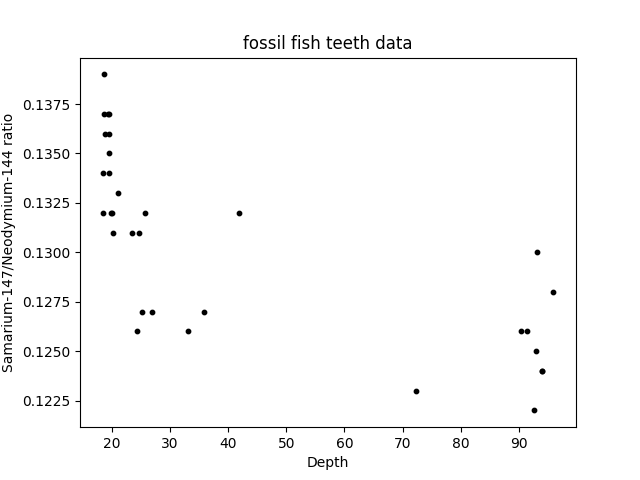
\includegraphics[width=\linewidth]{figs/fossil_fish_teeth}
	\caption{Sample data of Samarium-147/Neodymium-144 ratio in fossil fish teeth.}
	\label{fig:fossil_fish_teeth}
\end{figure}


For larger values of $n$ this gets increasingly difficult\footnote{For higher dimensionality we have to use some projection. Depending on the chosen projection the interpretation changes, therefore it is difficult to interpret the resulting image.}. PCA tries to solve this problem by transforming the data in such a way that the most interesting features are in the first few axis of the transformed $m$ dimensional space. This makes it easy to look at a low dimension representation of the data, without loosing much information.

An example of PCA being applied to the fossil fish teeth data can be seen in figure~\ref{fig:pca_example}. In the top figure the original data and the direction of the first two PCs in relation to the two axis is shown. The bottom figure depicts the transformed data.

\begin{figure}
	\centering
	\begin{subfigure}{0.5\textwidth}
		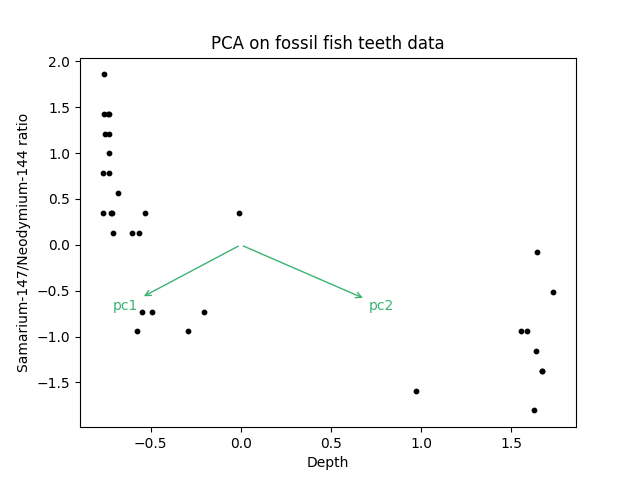
\includegraphics[width=\textwidth]{figs/fossil_fish_teeth_with_pcs}
		\caption{Original data and direction of the two PCs in relation to the ratio and depth.}
		\label{fig:fossil_fish_teeth_with_pcs}
	\end{subfigure}
	\hfill
	\begin{subfigure}{0.5\textwidth}
		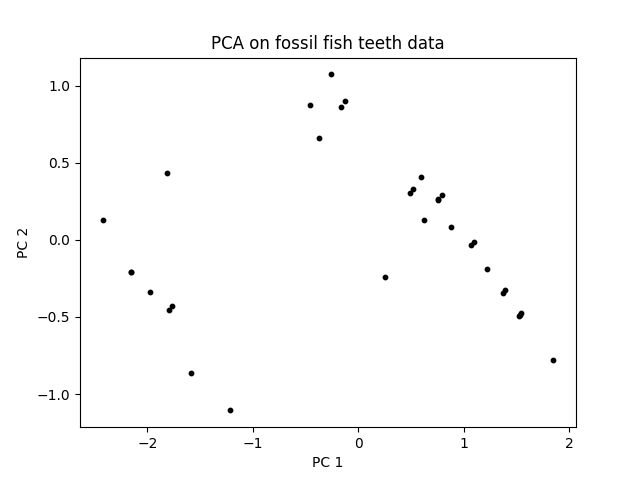
\includegraphics[width=\textwidth]{figs/pca_of_fossil_fish_teeth}
		\caption{Fossil teeth data after being transformed by PCA.}
		\label{fig:pca_of_fossil_fish_teeth}
	\end{subfigure}
	
	\caption{Example application of PCA on fossil fish teeth data.}
	\label{fig:pca_example}
\end{figure}

Now we derive how to compute PCA. First we formulate a goal and define some assumptions.

We assume that the most interesting features are those that have a large variance\footnote{This assumption can be false. For data where the noise has a larger variance than the feature we are trying to observe PCA fails because this assumption is not met.}. Our goal is to find a transformation into new coordinates such that:
\begin{itemize}
	\item the variance in the each axis is as large as possible.
	\item the axis are all orthogonal to each other.
	\item the axis are sorted (descending) by the variance in the axis.
\end{itemize}

From this we gather that another assumption is, that the axis are orthogonal.

One way to achieve the goal is as follows:
\begin{enumerate}
	\item Find the direction which maximizes the variance.
	\item Save this direction as the next axis.
	\item Determine the subspace that is orthogonal to all axis we found so far.
	\item If the subspace is non-trivial start at the first step again.
	\item If the subspace is trivial we have found all axis.
\end{enumerate}

Let $\mathbf{X} \in \mathbb{R}^{m\times n}$ be the data matrix. We want to find some orthonormal matrix $\mathbf{P}$ such that $\mathbf{Y}:=\mathbf{PX}$ has a diagonal covariance matrix $\mathbf{C}_{\mathbf{Y}}$.

\begin{align*}
	\mathbf{C}_{\mathbf{Y}} = \frac{1}{n}\mathbf{YY}^T = \frac{1}{n}(\mathbf{PX})(\mathbf{PX})^T = \frac{1}{n}\mathbf{PX}\mathbf{X}^T\mathbf{P}^T =\\
	= \mathbf{P}(\frac{1}{n}\mathbf{X}\mathbf{X}^T)\mathbf{P}^T = \mathbf{P}\mathbf{C}_\mathbf{X}\mathbf{P}^T
\end{align*}

The covariance matrix $\mathbf{C}_\mathbf{X}$ is symmetric and therefore has a decomposition into an orthongonal Matrix of eigenvectors $\mathbf{E}$ and a diagonal matrix of eigenvalues $\mathbf{D}$. We choose $\mathbf{P}=\mathbf{E}^T$. From lemma~\ref{lem:inverse_is_transpose} it follows that $\mathbf{E}^{-1} = \mathbf{E}^T$.

\begin{align*}
	\mathbf{P}\mathbf{C}_\mathbf{X}\mathbf{P}^T = \mathbf{P}(\mathbf{EDE}^{-1})\mathbf{P}^T = \mathbf{P}(\mathbf{EDE}^{T})\mathbf{P}^T =\\
	\mathbf{P}(\mathbf{P}^T\mathbf{DP})\mathbf{P}^T = (\mathbf{P}\mathbf{P}^T)\mathbf{D}(\mathbf{P}\mathbf{P}^T) =\\
	(\mathbf{P}\mathbf{P}^{-1})\mathbf{D}(\mathbf{P}\mathbf{P}^{-1}) = \mathbf{D}
\end{align*}

In summary $\mathbf{Y}$ has a diagonal covariance matrix if we choose $\mathbf{Y} = \mathbf{E}^T\mathbf{X}$, where $\mathbf{E}$ is the matrix of eigenvectors of $\mathbf{C}_\mathbf{X}$. The eigenvectors are the PCs and the eigenvalues are the variance in each new axis.

As pseudo code we get the following program for calculating the PCA:

\begin{algorithm}
	\caption{Principal Component Analysis}\label{alg:pca}
	\begin{algorithmic}
		\Require matrix $X \in \mathbb{R}^{m\times n}$
		\State Normalize each row in the matrix $X$
		\State Calculate the covariance matrix $C_{X}$
		\State Calculate the eigenvalues and eigenvectors of $C_{X}$
		\State Sort the eigenvalues
		\State Return sorted eigenvalues and corresponding eigenvectors
	\end{algorithmic}
\end{algorithm}

What happens if we skip the step in which we normalize each row in the matrix? A big variance is interpreted by the PCA algorithm as much information, thus the variance of the variables have an impact on how ''important'' the variable is deemed. As we do not want to prioritize certain variables we avoid this behavior by normalizing the data beforehand.

\section{Sleep Stages and EEG Data}
\label{sec:sleep_stages_and_eeg_data}

\section{Data and Algorithm}
\label{sec:data_and_algorithm}

\begin{enumerate}
	\item subdivide eeg signals in the temporal domain
	\item apply fft transforming into frequency domain
	\item pca
	\item achive dimensinality reduction
	\item classification of sleep stages
	\item visulisation
\end{enumerate}

\section{Results}
\label{sec:results}

\section{Conclusion}
\label{sec:conclusion}

\bibliographystyle{plain}
\bibliography{document}

\end{document}
